%!TEX root = project.tex

\chapter*{About this project}
\paragraph{Abstract}
Brendan Keane is an experienced chef working in Galway city for many years. He identified a problem that he and many other chefs, cooks and food management staff faced daily and decided he was going to improve it.
He thought of a creating a better digital based system to improve upon the current paper based system. Being former student of Galway Mayo Institute of Technology(GMIT) he returned to the computing department with his idea.
The current system used by all premises that handle and prepare food is time consuming and the staff are constantly minding paperwork. These premises must legally fill these forms creating problems between management and staff if not completed.
The client’s idea was to reduce the amount of time wasted filling paper work. He hopes that food handling premises can adopt and use his system to manage their forms and improve their productivity. The client observed that most staff carried their phones around with them and an App could be used to complete the forms much faster and easier. The client also wanted to be able to analyse the data.


\paragraph{Authors}
The author of this project is Martin Coleman. Martin is a graduate of the BSc in Computing in Software Development in 2016. Currently he is pursuing a BSc(honours) in Computing in Software Development. Martin has an interest in computing, programming and various other technologies. Martin is always interested in improving his programming skills and knowledge.

\chapter{Introduction}
This chapter introduces the project and the client. It discusses the origins of the project idea and the aims of the project.

\section{Client}
Brendan Keane is an experienced chef working in Galway city for many years. He identified a problem that he and many other chefs, cooks and food management staff faced daily and decided he was going to improve it.

He thought of a creating a better digital based system to improve upon the current paper based system. Being former student of Galway Mayo Institute of Technology(GMIT) he returned to the computing department with his idea.

\section{Client’s Problem}
The current system used by all premises that handle and prepare food is time consuming and the staff are constantly minding paperwork. These premises must legally fill these forms creating problems between management and staff if not completed.

\section{Client’s Idea}
The client’s idea was to reduce the amount of time wasted filling paper work. He hopes that food handling premises can adopt and use his system to manage their forms and improve their productivity. The client observed that most staff carried their phones around with them and an App could be used to complete the forms much faster and easier. The client also wanted to be able to analyse the data.

\section{Project Aim}
To create both Web and Mobile based Applications that connect to a comprehensive cloud based system that manages data for its users.\\ \\
With knowledge of the client and the problem, Chapter two will delve into the project itself. It discusses different elements of the project in detail.


\chapter{Context}
This chapter discusses the project. It covers areas such as deliverables that were by set by the client at the start to other areas such as risk, scheduling and scope that had to accessed after brief was received.

\section{Objectives}
The objectives were decided upon at the start of the project. They were decided upon after the initial meeting.\\

The objectives were as follows:

\begin{itemize}
\item To come to a mutual understanding of the project and understand the requirements of the project.
\item To research techniques and technologies to find the best solution to the project.
\item To design a system architecture that is the most suitable for the project.
\item To create a system and software capable of fulfilling all the requirements.
\end{itemize}

\section{Deliverables}
The deliverables were decided upon at the start of the project. They were derived from what the client wanted. \\

The deliverables were as follows:
\begin{itemize}
\item A cross platform mobile application for Android and Apple iOS.
\item A web application that allows users to view their saved forms.
\item A cloud service that stores the data and runs the servers.
\end{itemize}

\section{Source Code}
All the source code used in this project is available on GitHub. At the first link below you will find the source code for the mobile application. At the second link, you will find the source code for the web server and the API server.

Both repositories contain their own README.md file that has information about the project, how to setup the required environment and how to run both servers and build the mobile application.\\

Links to GitHub Repositories:

https://github.com/Martinc94/HACCPManagementApp

https://github.com/Martinc94/HACCPAPZ-Server


\section{Scope}
This project is about to designing and implementing a whole system to solve satisfy the client. It contains a mobile application, a web application, an API server, a database and a cloud server to connect and host the services for all the above.

The scope of the project is a similar level to a project that a customer might require in industry. Its requirements were achievable within the given time. The project contains many elements such as mobile, web, databases, user authentication, managing a cloud server, data analysis, data handling, transfer and manipulation. These elements combined cover a wide range of areas that are relevant to the course. The project has great room for expansion and many possibilities to implement.


\section{Relation to Degree}

The project related to the degree on many levels as it contains a wide spectrum of different technologies, problems and tasks that are covered on the course and are commonplace in industry. The project contains mobile and web front-ends, a back-end for handling data, an API for accessing the back-end, a database and a cloud server to handle all the parts mentioned above. \\

Some of the course modules that related to the project:

\begin{itemize}
\item Emerging Technologies.
\item Data Representation and Querying.
\item Mobile programming.
\item Database management systems.
\item Software Testing.
\item Internet application development.
\item Graphical User Interface and Web development.
\end{itemize}
	
\section{Minimum requirements}
The minimum requirements for the project were set as a worst-case situation for the project. The client was assured that he would receive a system that would satisfy these requirements. Even if a major problem slowed down development of the system it was felt that these requirements could be achieved. \\

The minimum requirements for the projects were:

\begin{itemize}
\item A cross platform mobile application for Android and Apple iOS.
\item A cloud service for storing data from mobile application.
\item A website to display stored data.
\item A database to store the data.
\item An API server to connect above services.
\end{itemize}

\section{Enhancements}
The possible enhancements to the project included some features the client wanted to be implemented in the system and some enhancements thought of with the project supervisor to improve the system. These enhancements were to be worked on after the minimum requirements were achieved. \\ 

The possible enhancements to the project were:
\begin{itemize}
\item Analysis of data for administrator use.
\item Graphical representation of data analysis.
\item Incorporation of Google maps for location services.
\item Take photos on mobile application and store on server.
\item Display photos alongside relevant forms.
\end{itemize}


\section{Risk}
The risks involved with the project were all the most common problems that could go wrong in the software development process. They were analysed and decided upon at the start of development so they could be monitored and avoided. \\

The risk involved in the project included:

\begin{itemize}
\item Miscommunication of requirements.
\item Incorrect or incompatible technologies being chosen.
\item Using new technologies.
\item System architecture and design.
\item Performance of various systems.
\item Organisation and work management.
\end{itemize}

\section{Security}
The project requires security on each component of the system. Sensitive data such as passwords being stored in the database must be protected. Access rights to user’s data and to different parts of the web application must also be protected. The API server must authorize who can access its HTTP methods.

\section{Scheduling}
The scheduling for the project had to be planned early to keep the development on schedule and make sure each deadline is met. Scheduling is an important element of software projects. Many failed projects can conclude that the main cause of failure was poor time management at early stages of development. \\

Early in the projects life cycle the scheduling will focus on requirements gathering.
\begin{itemize}
\item Requirements gathering.
\item Research on project and technologies.
\end{itemize}		


After the requirements are gathered, focus must change to the first milestone, the first prototype of the mobile application.
\begin{itemize}
\item Decision on technologies and start development.
\item Develop prototype mobile application.
\item Evaluate prototype and redesign if required.
\end{itemize}


When the mobile prototype is developed, the focus switches to the second milestone which is to get the server setup and communicating with the mobile application.
\begin{itemize}
\item Setup cloud server on azure.
\item Setup database on azure.
\item Start development of API server.
\item Working draft of API server and mobile app working.
\end{itemize}


Once the mobile application and server are communicating, the focus will be to start development on the web application.
\begin{itemize}
\item Start development of web application and server.
\item Prototype of web application. 
\end{itemize}	


When all the prototypes are working, the focus will change to creating a fully functioning version of them all.
\begin{itemize}
\item Working version of mobile application and API server.
\item Working version of Web application. 
\end{itemize}	


As full functionality of the system is achieved data analysis can begin.
\begin{itemize}
\item Start Analysis of data.
\end{itemize}


When all the enhancements are implemented the system and relevant extras can be handed over to the client.
\begin{itemize}
\item Delivery of finished project including mobile packages.
\end{itemize}
	
\section{Document Overview}
This rest of this document contains an in depth look at the development process.

Chapter three focuses on the methodologies that were researched and implemented in to the project. It includes both research and software development methodologies. It also discusses area such as project management, meetings and development tools.

Chapter four reviews in detail the technologies and architectures that were chosen for this project. It provides an insight as to why certain choices of technologies and architectures were chosen to help produce a system that is modern, adaptable and scalable.

Chapter five looks at the system design in fine detail. It talks about how the different elements interact together and how what role each element performed to produce the final system.

Chapter six talks about how the system was evaluated. This includes how the system was tested. The various forms of testing that were looked at include Unit, Integration, Functional, Usability and Acceptance testing.

Chapter Seven concludes the whole project. It provides an overall review of how the project went and any improvements that would be implemented if project was to be redeveloped.




\chapter{Methodologies}
This Chapter covers the different methodologies that were implemented in this project. It looks at the different types of research methodologies that were used such as Qualitative and Quantitative, different software development methodologies and why they were chosen. Other areas covered include testing, meetings, project management and development tools.

\section{Research methodology}
Firstly, the research methodology that was used in this project was Qualitative~\cite{newman1998qualitative}. Qualitative research is useful for studies at an individual level. It was important to gain an insight from the client’s perspective and to establish what requirements the client had. 

The main way that research was collected was from interviews and meetings with the client. This information helped to decide what had to be completed, what technologies were best for the project and what software methodology would be most suitable to use in the project.

Later in the projects life cycle Quantitative~\cite{newman1998qualitative} research was used. The Prototypes of the mobile and web applications were distributed by the client and he returned the feedback. This allowed us to gain valuable insight into what potential users thought about the applications. The feedback was used to make adjustments that improved the applications.

\section{Software Development methodology}
The software methodology that was used in this project was Extreme Programming (XP). Extreme Programming is a form of Agile software development. It became clear early that Agile would be the most suitable methodology to use. Agile allows for Incremental development, changing requirements, prototyping, sustainable development and close cooperation between business and developers. As there would be weekly meetings with client and supervisors being able to show progress would be a bonus.

There are many types of Agile methodologies. The decision was narrowed down to two types, Extreme Programming and Scrum. Extreme Programming was chosen over Scrum as Extreme Programming for the following reasons:
\begin{itemize}
\item Extreme Programming works in shorter iterations than Scrum.
\item Extreme Programming allows for continuous integration.
\item Extreme Programming works in strict priority order which allows most important features to be worked on and allows priority to be changed easily.
\item Extreme Programming recommends practices such as test driven development.
\end{itemize}	


Extreme Programming focuses on adaptability rather than predictability which was important in a project like this.
The values of Extreme Programming that were most relevant to the project:
\begin{itemize}
\item Communication between developer and client.
\item Simplicity of development.
\item Feedback from client/users.
\end{itemize}	

Software development process as described by Extreme Programming:
\begin{itemize}
\item Planning.
\item Analysis.
\item Design.
\item Development.
\item Testing.
\item Implementation.
\item Maintenance.
\end{itemize}	

XP Development Cycle~\cite{XPphoto}:

    \begin{center}    
      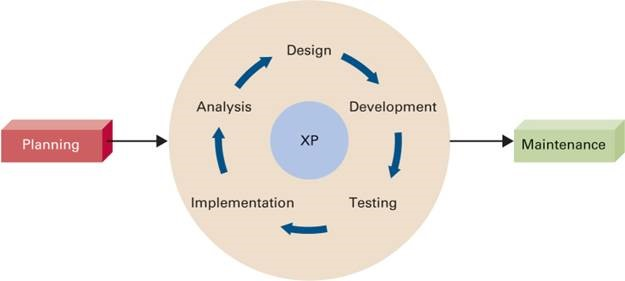
\includegraphics[width=100mm,scale=0.8]{img/XP.jpg}  
    \end{center}



\section{Testing}
The type of development chosen allowed for Test driven development. Test driven development allow for continuous testing to happen alongside development. Tests can be written before or after new code is written. Tests can be run before and after new code is added to test to see if new code performs as expected and on old code to make sure new code hasn't effected old code. \\

This type of testing suited the project as there were many iterations of the project. Testing frequently made sure new and old code worked each iteration. This also prevents bugs being embedded deep into the code. \\

Test Driven Development Cycle~\cite{TDDphoto}:
    \begin{center}    
      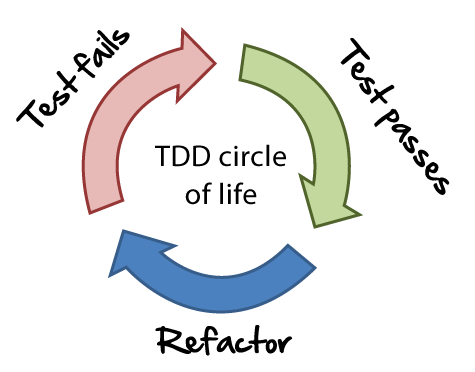
\includegraphics[width=80mm]{img/TDD.png}
    \end{center}

The main testing tool used during development was Postman~\cite{postman}. Postman allows users to share, test, document and monitor APIs. Users can vary requests and see results in an easy to use and manage environment.

\begin{center}    
    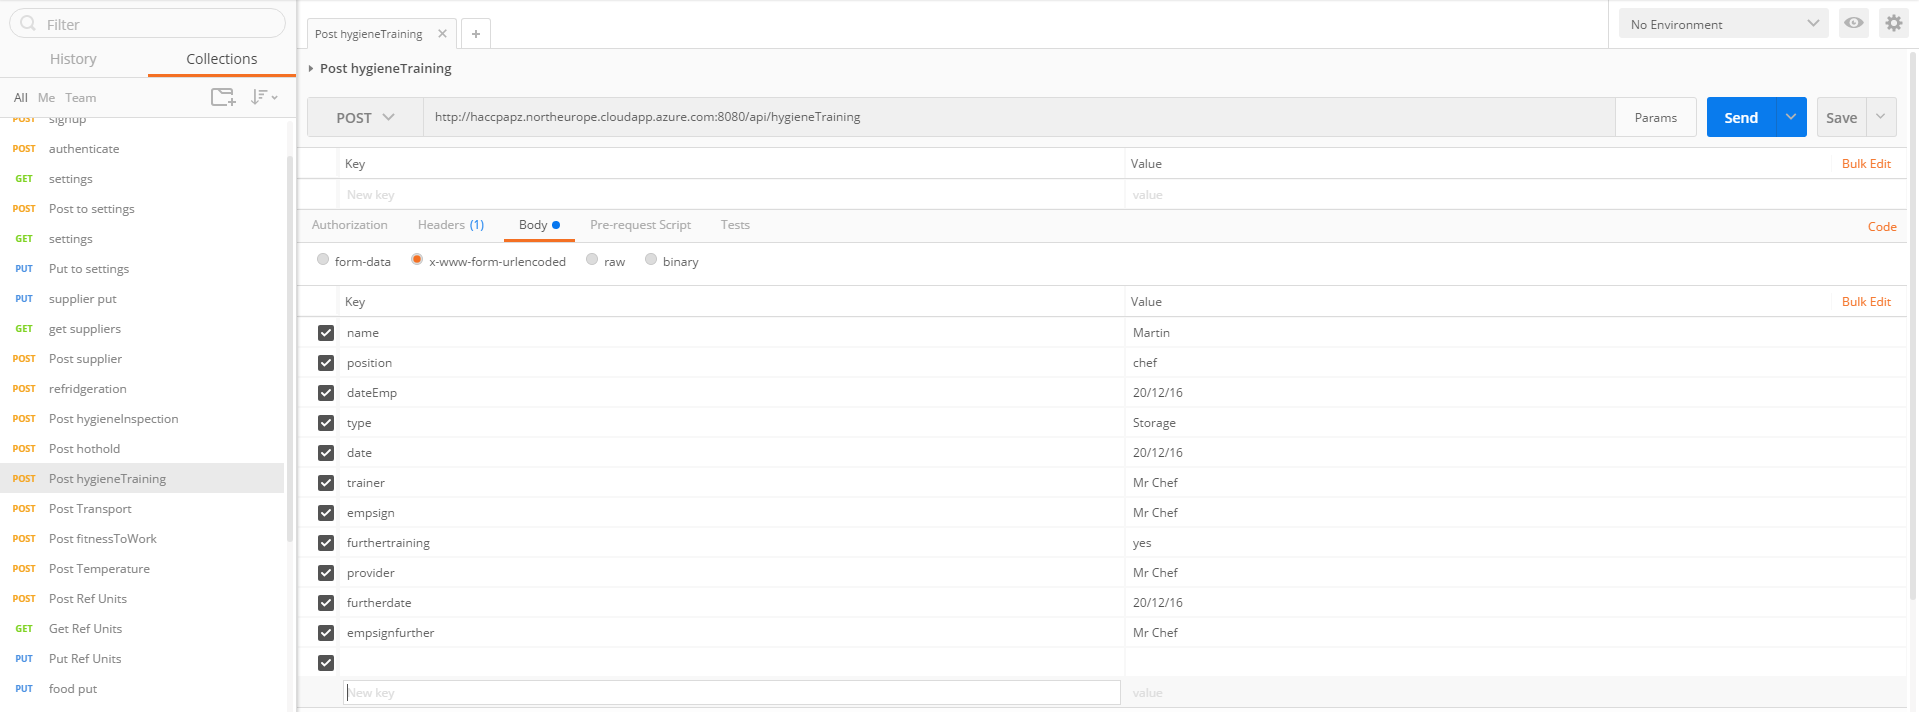
\includegraphics[width=140mm]{img/testing/postmanPost.png}
\end{center}


\section{Meetings}
Meeting were held weekly for the duration of the project. Meeting were with the project supervisors or the client.

Meetings consisted of:
\begin{itemize}
\item Progress Update.
\item Feedback on progress
\item Planning of next development iteration
\item Q and A on various project elements if required
\end{itemize}
	
\section{Project Management}
GitHub was used all throughout the development of this project. GitHub allows for version control of the project, back up of code and recording of documentation. GitHub makes progress tracking easier.

\section{Development tools}
The main integrated development environment(IDE) used was Visual Studio Code. This Integrated development environment was used because its support for typescript, HTML, JavaScript, JSON, integration of GitHub, IntelliSense and third-party extensions which provide extra support and many useful features.

\chapter{Technology Review}
This chapter discusses in detail all the various technologies that were incorporated into this project. The chapter also covers why the technologies for each component of the system were chosen and the benefits they provide.

\section{Overview}
The following are some of the most prevalent technologies were used in the development of this project:
\begin{itemize}
\item MEAN Stack
\item MongoDB
\item Express
\item Angular 1 and 2
\item Node 
\item Ionic
\item JSON
\item HTTP and REST
\end{itemize}
	
\section{Development}
The Mean stack is an open source JavaScript software stack. The MEAN stack consists of MongoDB as database, Express.js as a web application frame, AngularJS as a front-end framework, NodeJS as a JavaScript runtime. These four technologies combine so that both the client side and the server side can be written in the same language. MEAN stack is primarily used for designing dynamic web applications. Mean supports MVC (Model View Controller) architecture. MEAN stack passes JSON between the different components.

GitHub’s statistics suggest that the use of components of the MEAN stack are rising rapidly. Because all the components are open-source they are free to use and are constantly being updated and improving. \\

MEAN Stack~\cite{MEANphoto}:
    \begin{center}    
      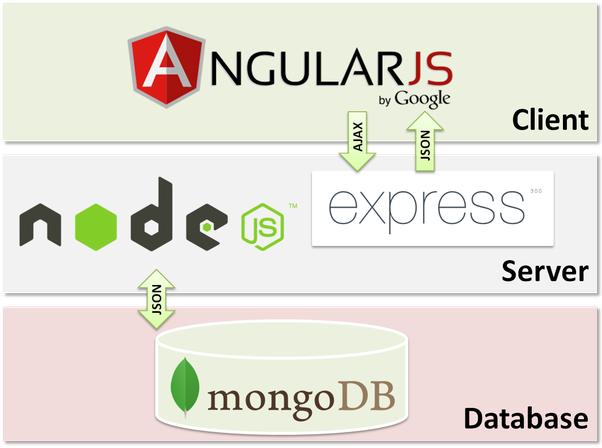
\includegraphics[width=80mm]{img/MEAN.png}
    \end{center}

\section{MongoDb}
MongoDB~\cite{mongoDB} is an open-source NoSQL database. It uses a document-based model to store data. The document based model it uses is JSON~\cite{JsonBson}. JSON uses key-value pairing to identify data. MongoDB uses collections and documents instead of using tables and rows like MySQL databases. Each MongoDB database is composed of collections and each collection is composed of documents. \\

\begin{center}    
    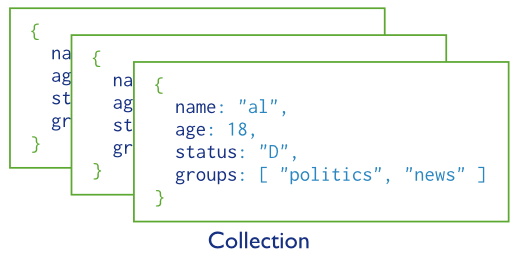
\includegraphics[width=80mm]{img/Collection.png}
\end{center}


Mongoose~\cite{Mongoose} provides an interface that connects MongoDB to NodeJS. Mongoose uses a schema based model. Mongoose handles query building, type casting, validation and business logic. \\

Example of Mongoose connecting to database, creating and saving a schema.

\begin{center}    
    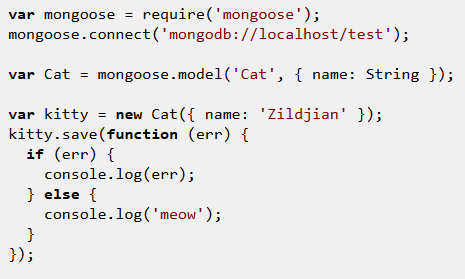
\includegraphics[width=80mm]{img/Mongoose.png}
\end{center}

This allows for fast saving of data. Each data model can be assigned its own schema and easily saved and retrieved. This allows for type safety of data if required.





\section{Express}
Express or Express.js~\cite{Express} is an open source web application framework for NodeJS. It provides set of features for web and mobile applications such as creating API’s. Express is a lightweight framework yet performs well. 

With Express you can get HTTP endpoints up and running fast and easy. Methods such as GET, POST, PUT, DELETE from the NodeJS HTTP module are all supported by express. \\

Example of how HTTP routes Can easily be setup:
\begin{center}    
    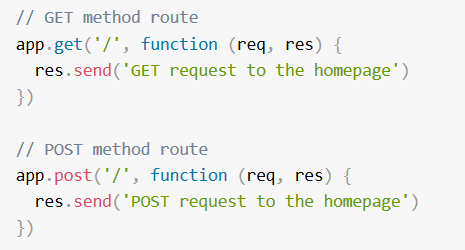
\includegraphics[width=100mm]{img/API.png}
\end{center}

This simple minimalistic design means that API routes can be setup and modified easily. This helps speed up development. 
\section{Angular}
Angular or AngularJS~\cite{Angular} is an open source JavaScript web and mobile application framework from Google. Angular lets developers to develop in a single language on multiple platforms, improves code reuse and performance. Angular is designed to be test friendly as components are separated from each other. 

Angular applications use dependency injection which means there is no main method to be managed. Dependency Injection lets you ask angular for an instance of a component and Angular will provide it for you. This makes angular more maintainable and because the components are injected they can be easily be removed or replaced.

Angular is designed to improve upon HTML (Hypertext Markup Language). Angular improves HTML by adding a dynamic element to it. Angular does this using client side architectures and data binding. The main architecture Angular implements is Model–View–Controller (MVC). 

\subsection{Model–View–Controller}
Model–View–Controller is a software architectural pattern used for designing user interfaces. It splits the software into three separate components, the View which is what the user sees, the Model which handles the data and updates the view and the controller which the user uses to manipulates the data in the Model. Each component should be loosely coupled to other components in the software. This allows for parallel development of components and components to be swapped in and out without affecting other parts of the system. 

For example, a class or object in the model gets information from database and renders it for the View to display to the user. The user uses the Controller to edit the data, the Controller modifies the data in the Model and the View Updates from the Model displaying the edited data to the user. \\

Model–View–Controller example~\cite{MVCphoto}:
\begin{center}    
    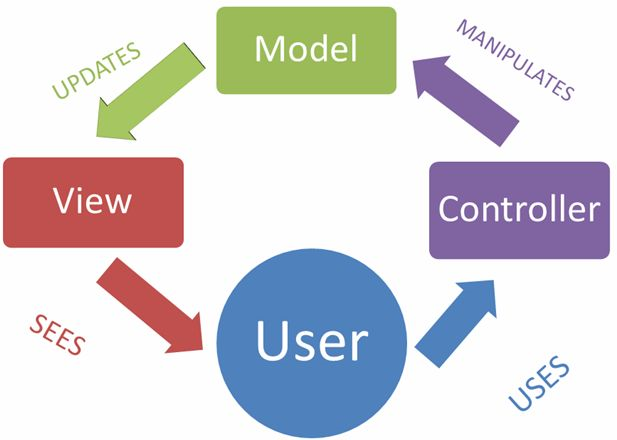
\includegraphics[width=80mm]{img/MVC.png}
\end{center}

\subsubsection{Model}
The Model is responsible for managing all the data and logic for the application such as manipulating data and getting data from external sources such as a server. It is also responsible for updating what the user sees in the View Component. 

\subsubsection{View}
The View is responsible for all the User Interface logic. It handles everything the user interacts with such as text boxes, forms etc. It updates itself with data from the Model.

\subsubsection{Controller}
The Controller acts a medium between the Model and the View. It lets the user interact with the Model to manipulate the data it contains.




\section{Angular 2}
Angular 2 is an improved version of Angular. It replaces JavaScript with Typescript. Angular 2 has all the benefits of Angular 1. \\

Angular 2 made the following improvements:
\begin{itemize}
\item Code structure is simplified and it easier to learn as there are less concepts.
\item Improves server-side speed.
\item Improved client-side performance as it uses server side rendering for faster viewing.
\item Provides support for newer and older browsers.
\end{itemize}

\subsection{TypeScript}
TypeScript~\cite{TypeScript} is a strict subset of JavaScript that is developed and maintained by Microsoft. Because it is derived from JavaScript, TypeScript can run any JavaScript code. 
TypeScript adds type safety and an object-oriented structure to the language. It uses many structures that common object-oriented based languages use such as Classes, constructors and Interfaces. 
TypeScript provides static typing through type annotations that enable type checking at runtime. Typescript is compiled to JavaScript which means it can run in any environment that supports JavaScript. \\

Example of Typescript class, interface, function and declaration of a class
\begin{center}    
    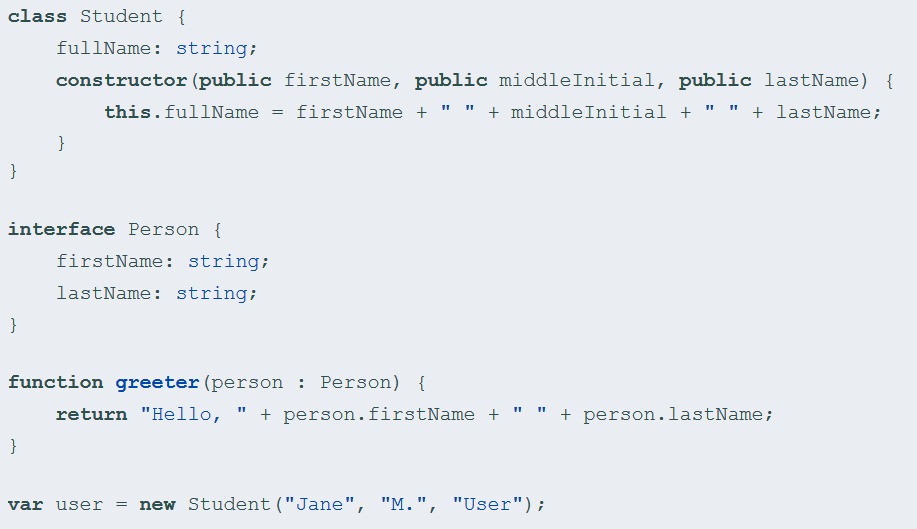
\includegraphics[width=110
    mm]{img/Typescript.png}
\end{center}

\section{Node}
NodeJS~\cite{Node} or Node is an open-source, asynchronous event driven JavaScript runtime that is designed to build network applications. Node is highly scalable and can handle many connections concurrently. Node interprets JavaScript using Google's V8 JavaScript engine. Node is lightweight yet powerful and is quickly growing in industry with large companies such as IBM, Microsoft, Netflix, PayPal, SAP, Yahoo and Cisco using it. As Node was designed with network applications in mind it implements HTTP. The use of HTTP means Node is suitable for building web frameworks on. \\ 

Example of a simple server in Node.
\begin{center}    
    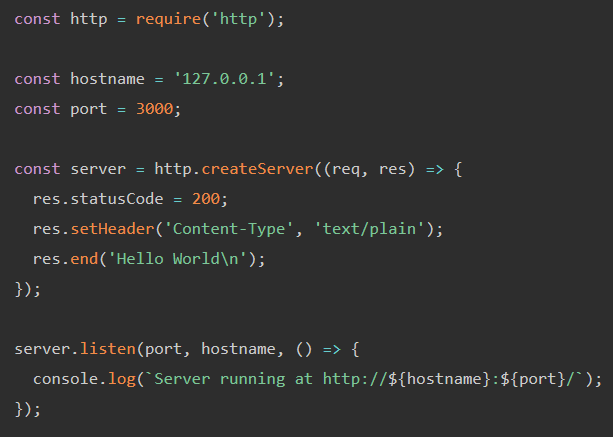
\includegraphics[width=140mm]{img/node.png}
\end{center}

\section{Ionic}
The Ionic Framework~\cite{Ionic} is an Open-source mobile application software development kit. It is built on top of Angular and Cordova. It builds mobile applications using web technologies like HTML and CSS. Ionic applications use the mobile devices web browser to run. Because of this, applications don’t have to be written in the devices native code meaning that Ionic applications can used to same code to run on multiple devices and operating systems such as Android and IOS.

\subsection{Apache Cordova}
Apache Cordova~\cite{Cordova} is a mobile application development framework that lets the native features of devices such as camera and location work with HTML. Cordova provides a wrapper to native APIs. These plugins can be installed by developers as required and allow developers to access the device's native accelerometer, geolocation, camera, file system and microphone etc. This greatly speeds up development as no knowledge of the native APIs are needed. Cordova supports a wide range of devices such as Android, Apple, Blackberry and Windows phone.

\section{JSON (JavaScript Object Notation)}
JavaScript Object Notation~\cite{Json} or JSON as its more commonly known is a syntax for storing and exchanging data. JSON is fast becoming industries most used data interchange format. JSON is Text based format which makes it easy for humans to both read and write.

JSON is lightweight which makes it easy to parse and generate for machines. It is preferred in most network applications as its less verbose than traditional methods such as XML (eXtensible Markup Language). JSON is based on JavaScript objects but because it is text based it is language independent. Because it is so easy to use and generate most common languages have adopted JSON. \\

JSON is designed from two structures:
\begin{itemize}
\item A name/value pair
\item Lists of pairs
\end{itemize}	

These are common data structures. Most common languages represent name/value pairs as objects or structs and represent lists as Arrays or sequences. This makes JSON interchangeable easily between languages and allows almost any language to be able to communicate to another language. \\

The values that JSON supports are:
\begin{itemize}
\item Strings
\item Numbers
\item Objects
\item Arrays
\item true
\item false
\item null
\end{itemize}	

Example of JSON name/value pairs:
\begin{center}    
    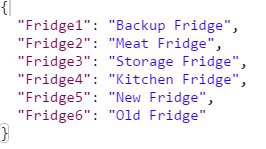
\includegraphics[width=80mm]{img/json.png}
\end{center}

JSON is used in many databases as its quick to store, retrieve and parse/load into applications. It reduces time taken by Database as it doesn't have to manipulate data, less verbose data can be sent and received faster and applications can easily parse the JSON data.

\section{HTTP}
HTTP~\cite{HTTP} (Hypertext Transfer Protocol) is the set of rules followed for transferring files over the internet. HTTP runs on top of the TCP/IP suite. TCP (Transmission Control Protocol) is the main internet protocol for data transfer. It combines well with the IP (Internet Protocol) to form the TCP/IP suite.

HTTP allows for the transfer of files such as text, images, videos and sound. \\

HTTP uses the following methods: 
\begin{itemize}
\item GET
\item POST
\item PUT
\item DELETE
\item HEAD
\item OPTIONS
\item CONNECT
\end{itemize}
	
These methods can be used to define what the request wants. The most commonly used Methods are GET and POST. GET requests data from a specified resource and POST submits data to a specified resource. e.g. Request wants to GET data or Request wants to Post image to server.


\section{REST (Representational State Transfer)}
REST~\cite{REST} (Representational State Transfer) or RESTful is a method of communication for computers systems over the internet. REST is an implementation of HTTP methods. REST uses the same methods of that HTTP uses such as GET, POST, PUT, DELETE etc. This allows applications to benefit from the same style of communication the internet uses.
REST is stateless. This means it doesn't keep track of sessions improving performance reliability and scalability. This allows servers to respond to requests quickly and to forget about it after. Because REST is web based, responses can be cached to speed them up. \\


Chapter five discusses how the above discussed technologies combine to create the system. The chapter discusses the role of each component and how the chosen technologies benefit the system.




\chapter{System Design}
This chapter discusses the system design in detail. It talks about how the various components of the system such as mobile application and API server link together to create the system design. The chapter also covers the roles each component performs for the system.

\section{Overview}
The system consists of three elements working together, a Mobile application, a Web application and an Application Programming Interface. To get these separate elements working together a software architectural pattern had to be followed. After researching many different frameworks and technologies the decision was made to base the design on the MEAN stack. 

This decision was largely influenced by the decision to use the Ionic framework. The Ionic framework uses Angular.js which is one element of the MEAN stack. The Ionic framework was chosen for the mobile application as it allowed the application to be developed once and be deployed on various mobile operating systems.

Applying the MEAN design to the rest of the project was a good idea as it meant that most of the technologies were JavaScript based. This meant that once a strong understanding of JavaScript frameworks was gained the expertise was passed onto the next element of the project speeding up development as new technologies hadn't to be learned from scratch. Because all the technologies are of a similar origin there are less compatibility issues than if other technologies were used.

\section{Mobile Application}
Firstly the mobile application was designed as this was what the client felt was most important part of the system for him. The main objectives of the mobile application were to create text forms, take and add pictures to relevant forms, store pre-programmable user settings and be cross platform for Apple IOS and Android. The decision to use ionic was made as research showed it was cross platform and it supported plugins for working with native camera.

The mobile application consists of login and sign up pages, home page, settings page and various form pages.
\begin{itemize}
\item The login and sign up pages handle Authentication and signing up to use the system.
\item The home page links to other pages when logged in.
\item The settings page handles editing and saving user defined settings such as foods and suppliers.
\item The various form pages handle creating and handling form objects.
\end{itemize}	

\begin{center}    
    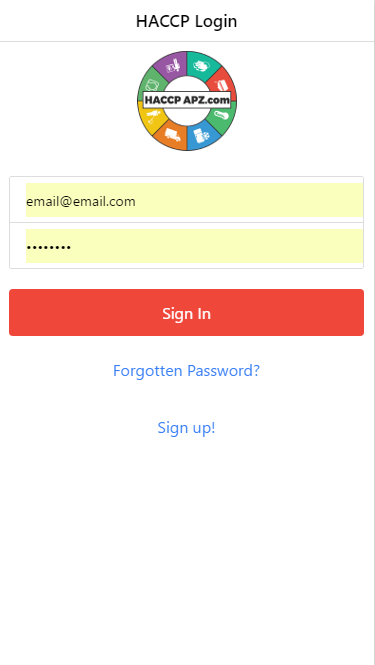
\includegraphics[width=40mm]{img/mobile/login.png}
    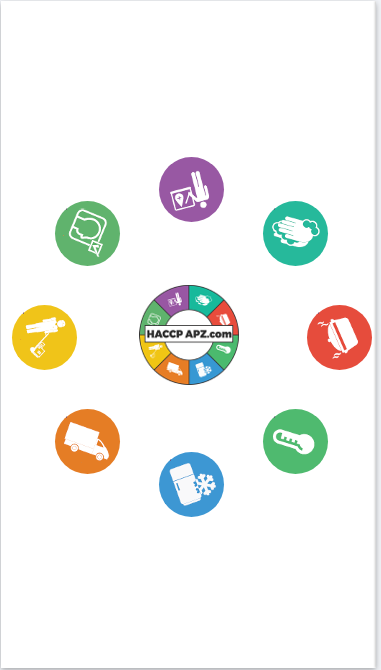
\includegraphics[width=40mm]{img/mobile/menu.png}
    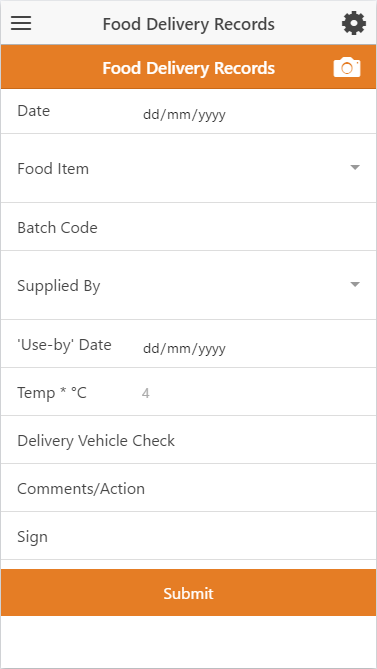
\includegraphics[width=40mm]{img/mobile/foodDeliForm.png}
\end{center}

The main role of the mobile application is to manage the forms the user creates and to communicate with the server. The applications roles include form adding a geolocation if relevant to forms, pushing data to and pulling data from the server, saving form if no data or Internet connection is available and handling Authentication. The mobile application is the main provider of data to the server. The data generated is in JSON format.

\section{Cloud Server}
The server is the core of the system. It’s the link between the mobile and web applications. It main role is hosting the services that the other elements of the project depend upon. 
It was decided to use Windows Server to speed up the development process as it was previously taught in the course and because the local development work was done on a Windows 10 machine it would minimise compatibility issues when moving from local test server to the cloud. 
The system is hosted on the Windows Azure platform as this was provided by the client.

\subsection{API Server}
The API server handles communication throughout the server. It is responsible for handling Authentication and data. The API handles storing data sent to it and sending data when requested. The server also handles any manipulation if data that is required.

NodeJS was chosen to run the API server at it is lightweight, scalable and reliable. Node can handle requests with speed and is easily testable with the Postman application.

The API server also provides data analysis to the web application. It is responsible for analysing and manipulating the data according to the request’s parameters. Node was a good choice for this as it’s a JavaScript runtime it was designed to work with JavaScript and JSON. The server could receive the request, manipulate the data and return the request in a fast time as it wasn't depending or waiting on an external program to do the work.

Using a RESTful design meant that the server didn't have to worry about managing session. This allowed the server to perform faster. It also provided API routing using HTTP method calls. All any application needs to access the API is standard HTTP. This allowed for simpler testing and design of web and mobile applications as they didn't require complicated setup to communicate with the API.

\subsection{Database}
The chosen database was MongoDB. MongoDB was chosen because it stores data in JSON format and because of Mongoose. Mongoose allows Node to query the database easily and add structure to the data in the form of schemas. This is particularly useful if data is required to be in an exact format. MongoDB also allowed the storage of photos which meant MongoDB was the only database that was needed.

\subsection{Web Application Server}
The cloud server also has the job of hosting the web application server. The web application is written in Angular 2. Angular adds makes HTML pages dynamic. Angular can communicate with the API to get the information its pages require.

The application is running on the same cloud to reduce any latency but if required the server is designed to run from any IP and contact the API server remotely. This could be useful if multiple instances of the application server are needed to be served in different locations in the future adding scalability.

System Architecture:
\begin{center}    
    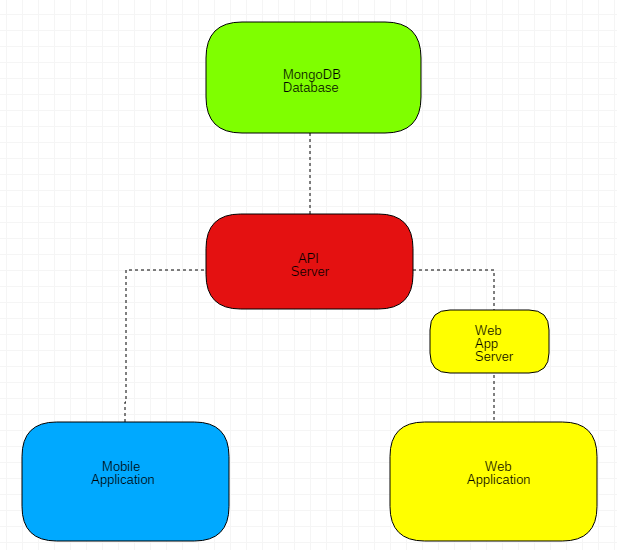
\includegraphics[width=100mm]{img/architecture.png}
\end{center}

\section{Web Application}
The web application was the last part of the application designed. This was useful as an understanding of all the data that was going to be displayed was had. The application could be designed to work around the data rather than changing the data to suit the website.

The main objectives of the web application were to display the gathered data stored in the database from the mobile application back to the user and to create queries and display the result of the analysis of the data to the user. \\

The web application consists of login page, home page, about page, settings page, user dashboard, data analysis pages and various form pages.
\begin{itemize}
\item The login page handles Authentication of users.
\item The user dashboard links to other pages when logged in and displays user information.
\item The settings page displays the user defined settings such as foods and suppliers.
\item The various form pages display the data from the database.
\item The data analysis pages let Administrators query and view analysis of data.
\end{itemize}

\begin{center}    
    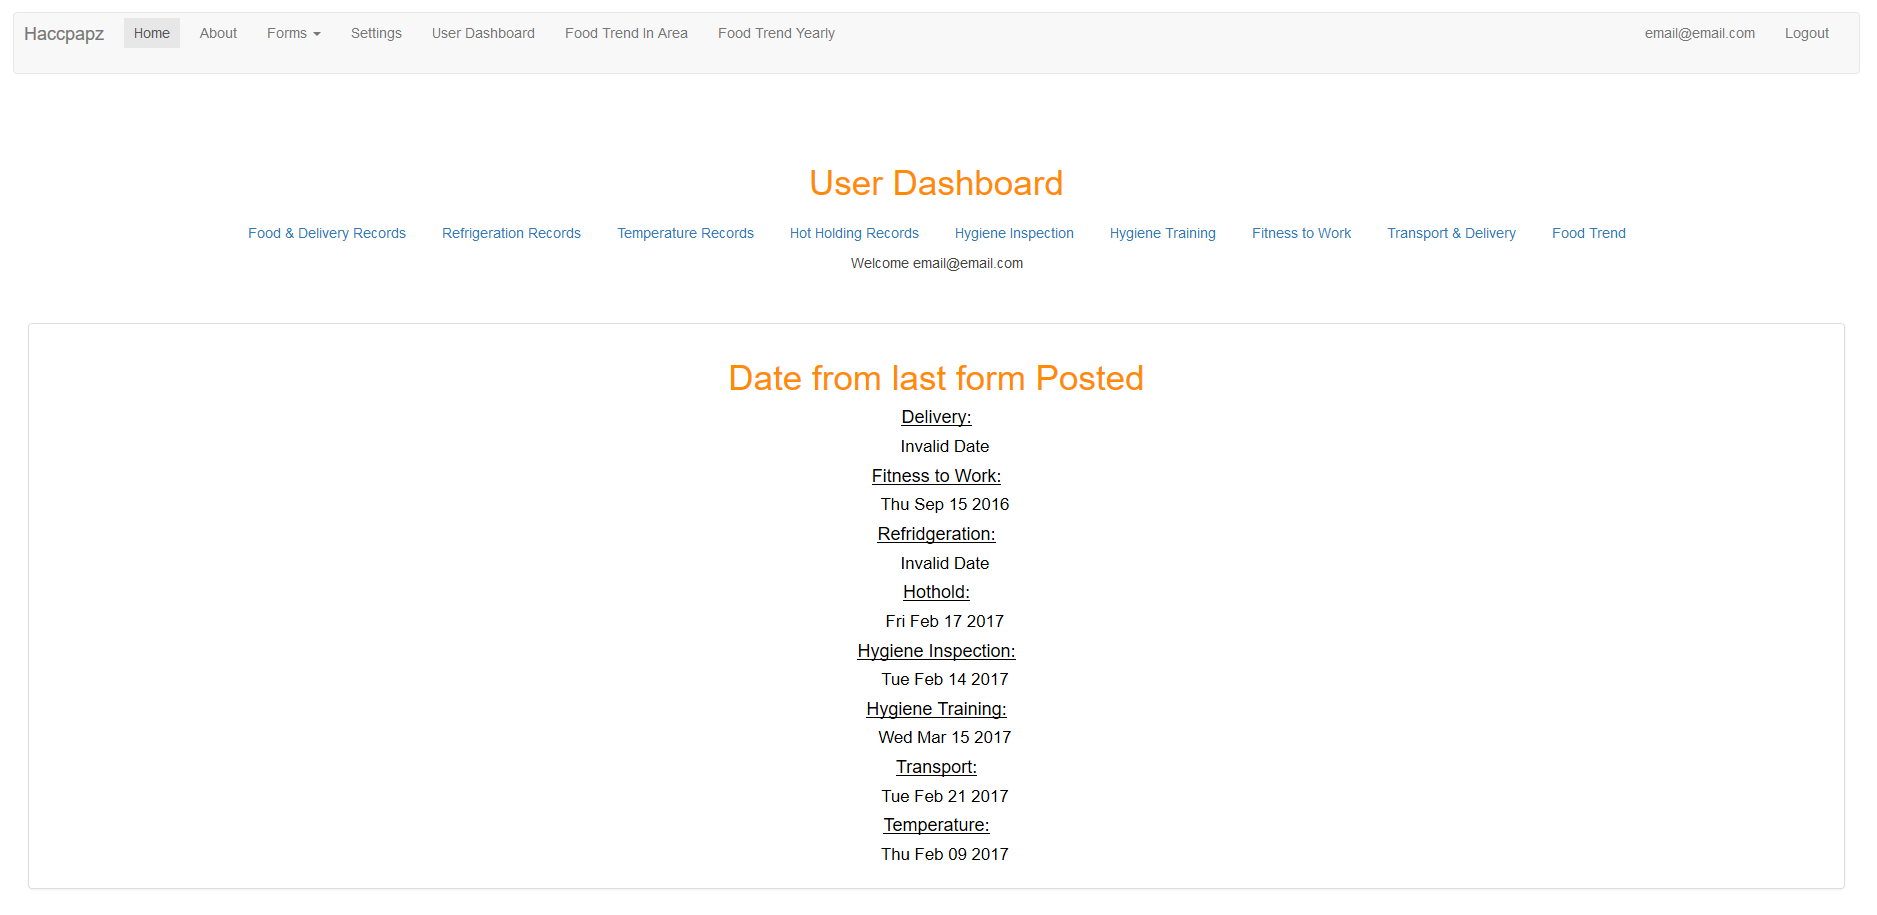
\includegraphics[width=140mm]{img/web/dashboard.png}
\end{center}

The choice to use Angular 2 was useful as Angular could manage requests, responses, Authentication of users and manipulation of data. 

Angular could provide and revoke access of different users to different pages. Users can only see their own data and cannot access pages without being logged in. Only administrators can perform analysis on the data. If an unauthorized user attempts to access a page they don’t have permission for they will be redirected to the homepage or the login page.

This application uses the Observables from the RxJS (Reactive Extensions for JavaScript) library in combination with the HTTP requests to get and handle data from the API. Observables improve on Promises which are commonly used in angular to get data. While Promises are only called once and return a single value Observables can handle multiple values over varied times. Observables can also be cancelled while Promises cannot be cancelled.\\

Example of an observable getting a collection of forms of type Hothold:
\begin{center}    
    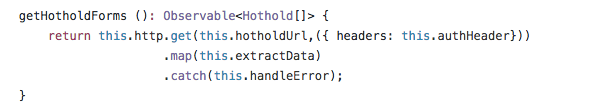
\includegraphics[width=140mm]{img/observable.png}
\end{center}

Angular also manages many powerful features such as Geo-location and Maps very well. The data analysis pages had to return the location of the search in its query. Angular gets the location of the user from the browser. \\

Example of code getting location when page initialises:
\begin{center}    
    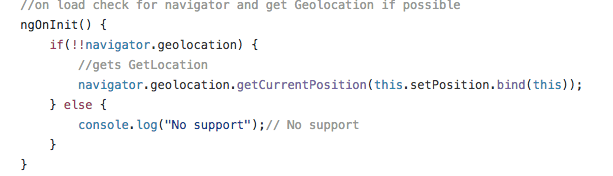
\includegraphics[width=140mm]{img/geo.png}
\end{center}

To allow the user to search from a different location Google maps was incorporated into the project. A map and location marker was added to the page. When used in combination with the browser geolocation the marker was placed at the user’s current location if location was allowed and the user could move the marker to select the location to query from. \\
 
Example of Google Map embedded in HTML:
\begin{center}    
    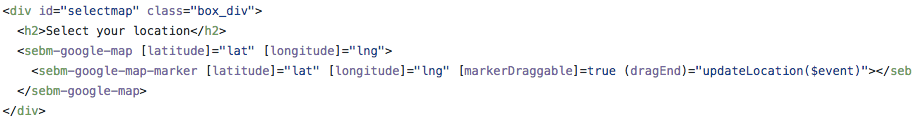
\includegraphics[width=170mm]{img/map.png}
\end{center}

Food Trend page: \\
\begin{center}    
    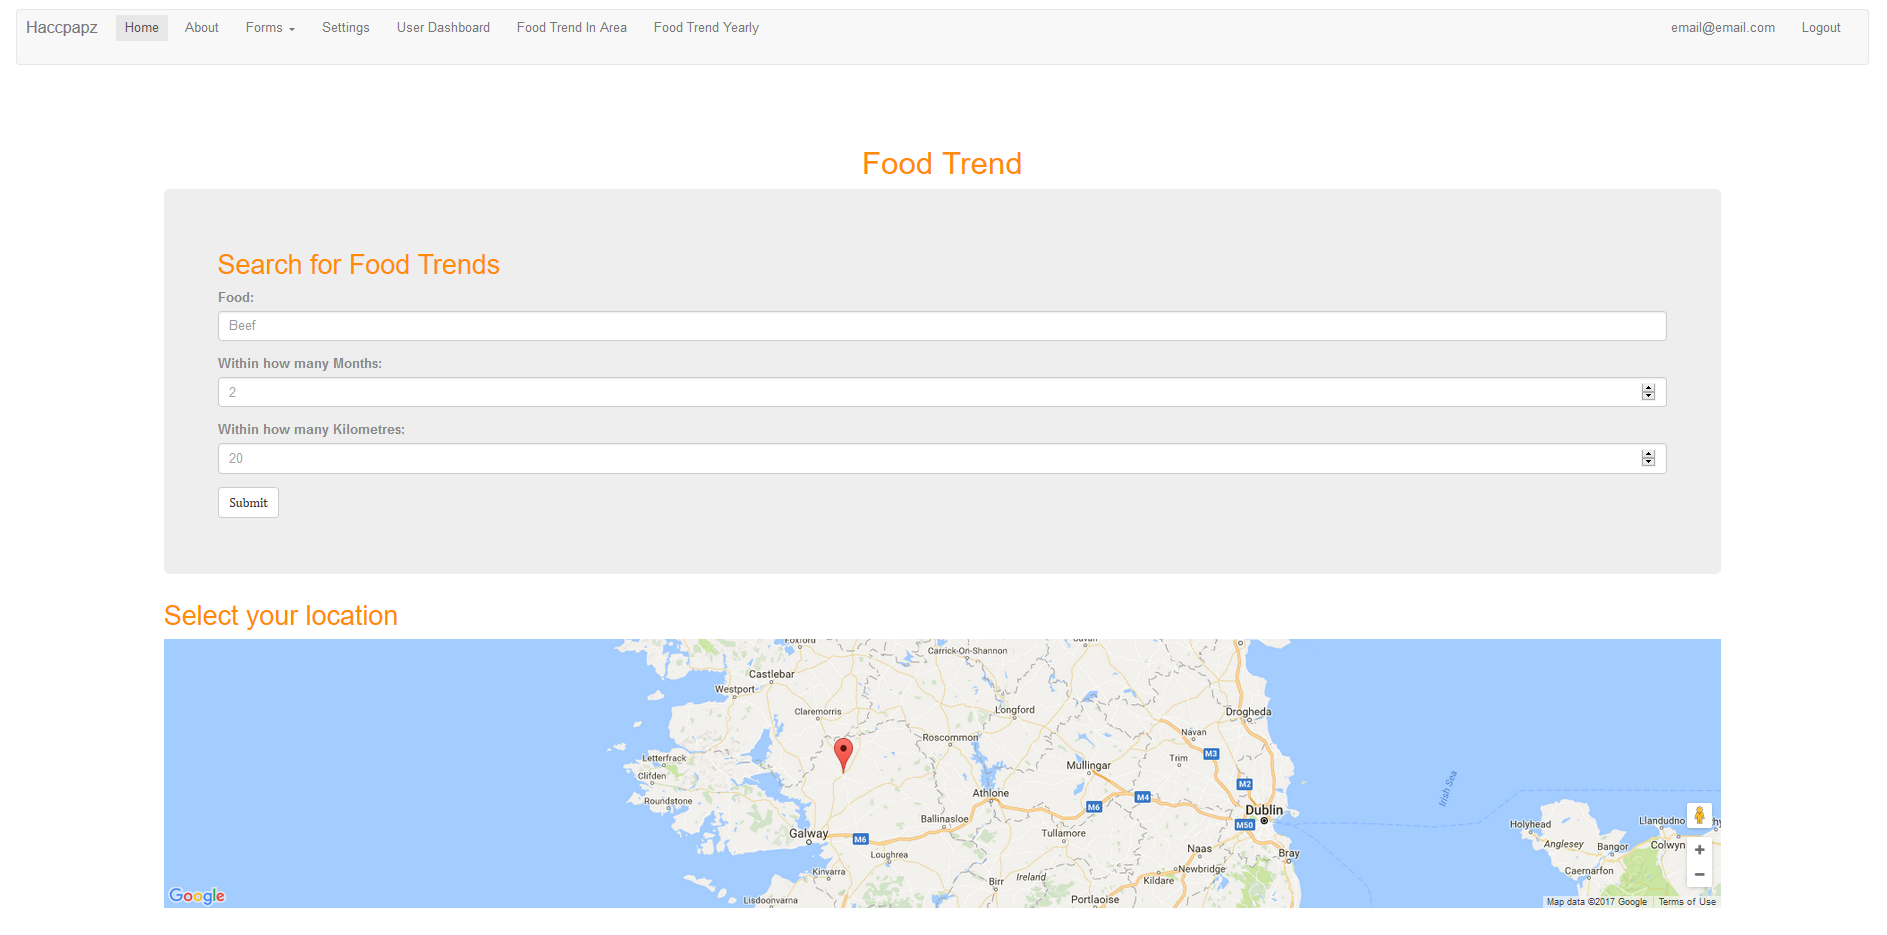
\includegraphics[width=140mm]{img/web/foodtrend.png}
\end{center}

Results map:
\begin{center}    
    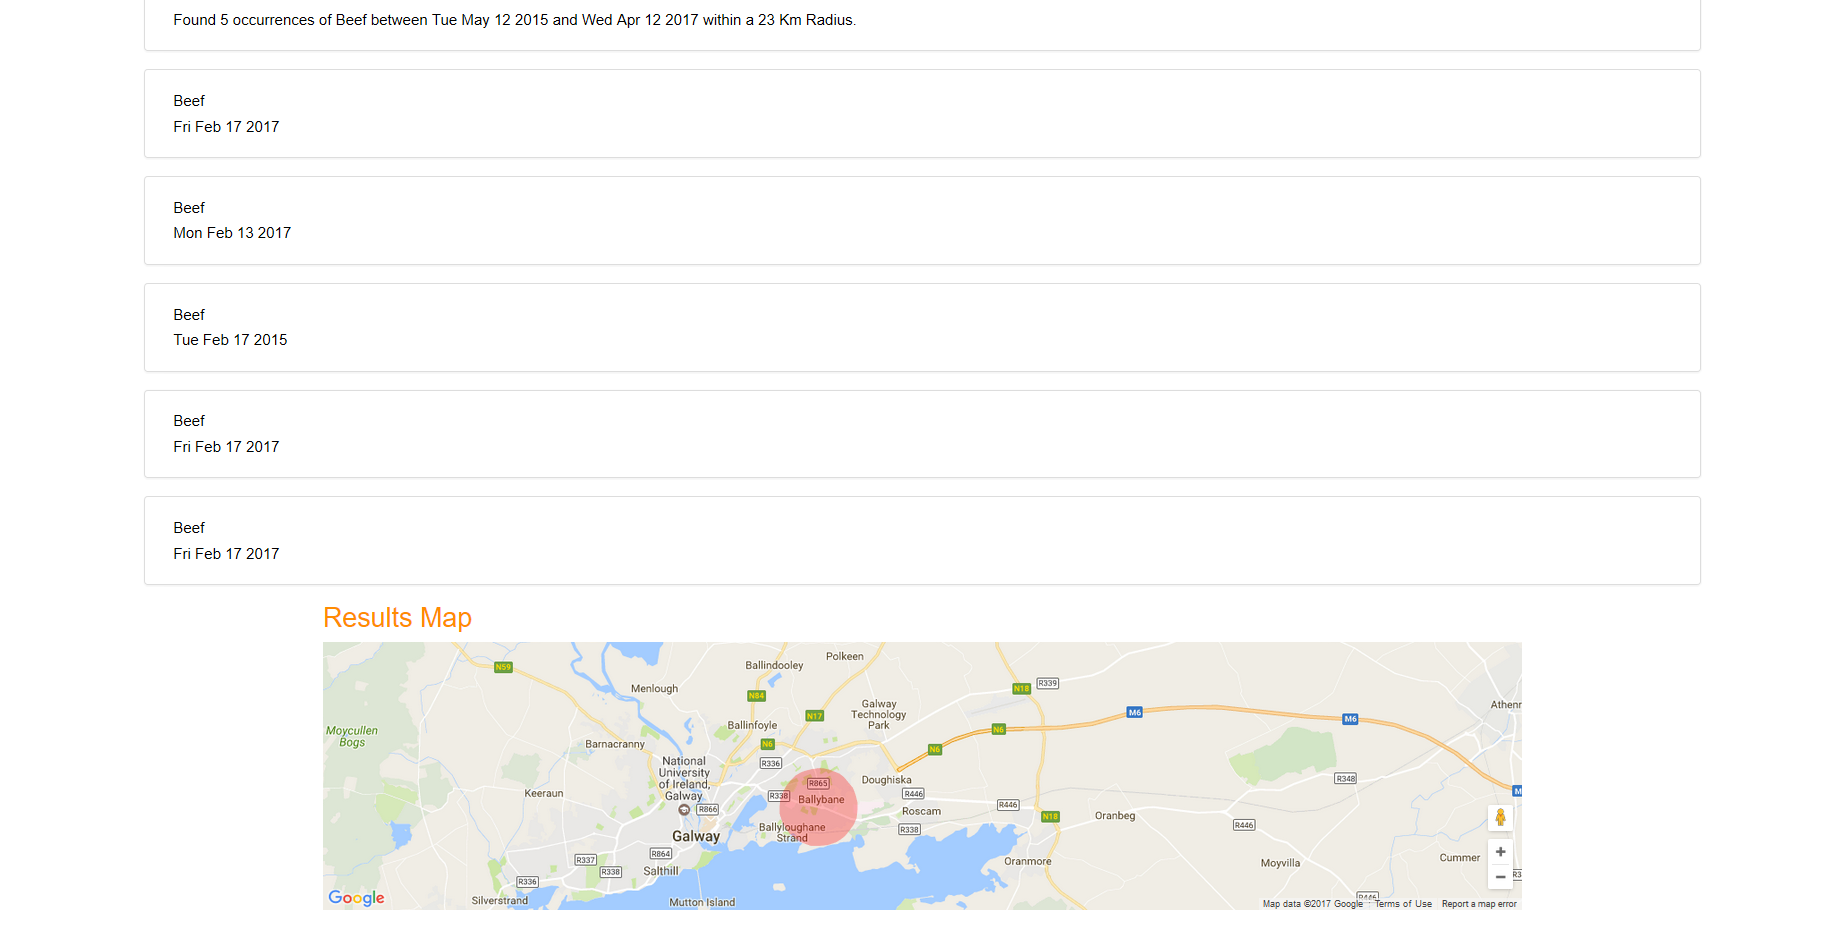
\includegraphics[width=140mm]{img/web/trendres.png}
\end{center}

Results bar chart:
\begin{center}    
    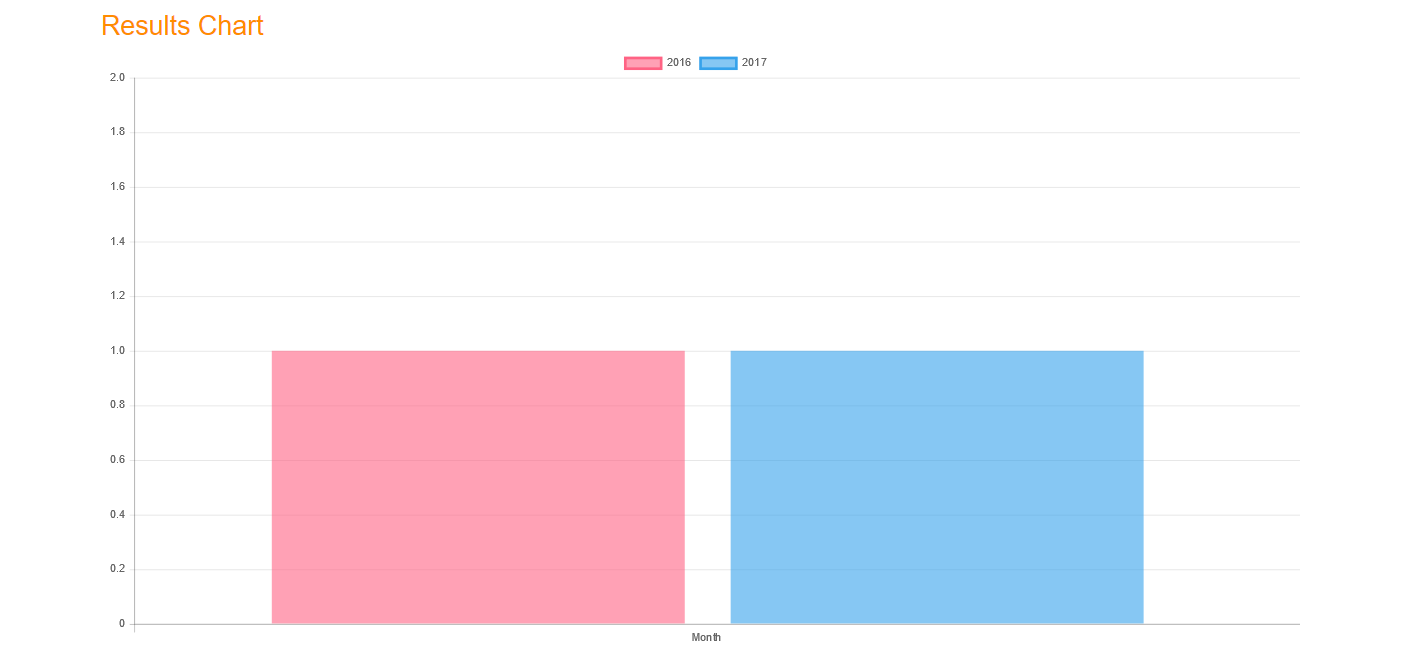
\includegraphics[width=140mm]{img/web/yearly.png}
\end{center}

Chapter six discusses how the system was evaluated. It discusses the various types of testing that was performed to make sure the system met requirements.

\chapter{System Evaluation}
This chapter discusses the various types of tests that were performed throughout the development life cycle to ensure software quality and that the requirement for the project were met.

\section{Overview}
The system was designed with test driven development in mind. As each unit of code as written relevant test were ran or new tests written if needed. Because test driven development was used during this project a lot of bugs were caught at an early stage and weren't built into the system. \\

The types of testing used included:
\begin{itemize}
\item Unit testing
\item Integration testing
\item Functional testing
\item Usability testing
\item Acceptance testing
\end{itemize}

\section{Unit Testing}
As each unit of code such as a HTTP Method was finished it was tested using the Postman~\cite{postman} application. Postman could send a request and view the result. The results could be examined to see if it passed test.

\begin{center}    
    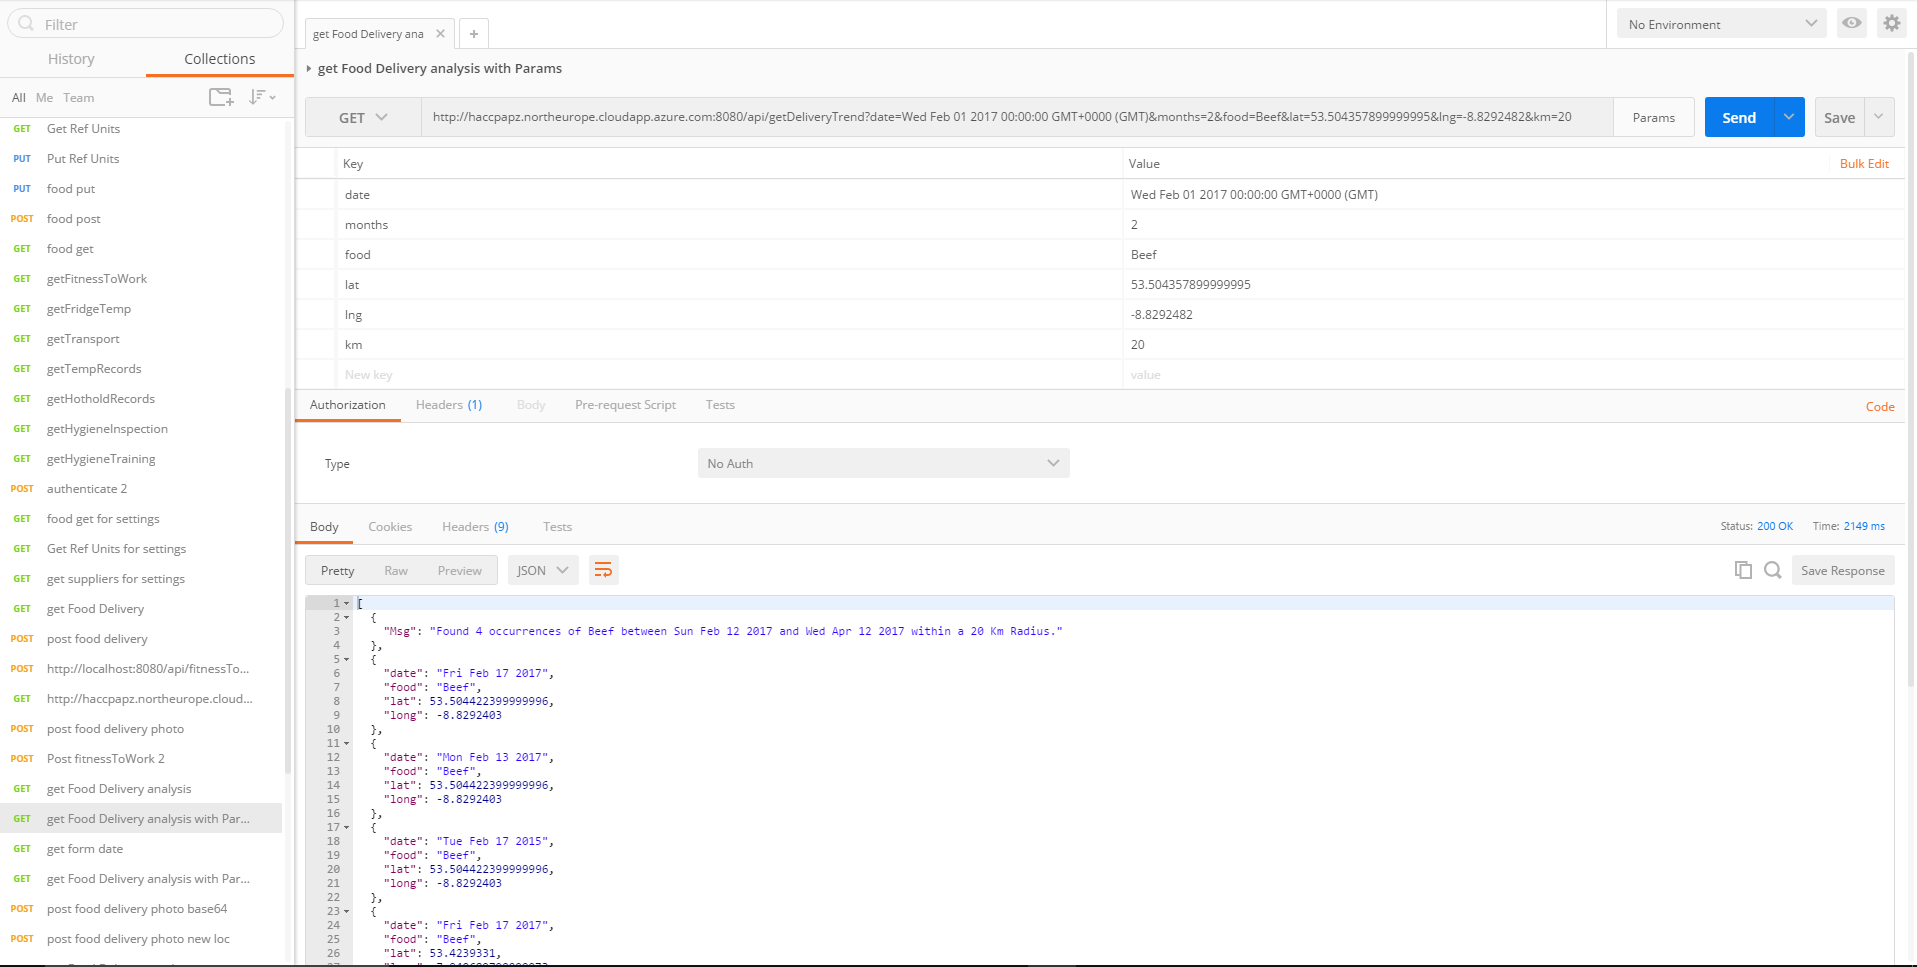
\includegraphics[width=140mm]{img/testing/postmanGet.png}
\end{center}

\section{Integration Testing}
When new components were added to the system tests were ran to see if any other components were affected by the changes. The whole system was tested to see how well the different components worked together.

\section{Functional Testing}
Each section of the system had its own functional tests to see if it was running as intended.

\subsection{Mobile Application}
The tests for the mobile application were:

\begin{itemize}
\item User can login.
\item User can sign-up.
\item User can access each form page from menu.
\item Each form page submits data when submit button clicked.
\item User can view, edit and submit settings to server from settings page.
\item User can take photo and submit photos with form if relevant to form.
\item User can submit forms saved in local storage from settings page.
\end{itemize}

\subsection{Web Application}
The tests for the web application were:

\begin{itemize}
\item User can login.
\item User will be redirected if not logged in.
\item Only administrators can access Data analysis pages.
\item Each form page can view its relevant forms from the logged in user.
\item User dashboard displays last date for each form submitted.
\item Administrator can enter food, date and range on food analysis page.
\item Food location shows up on results map on food analysis page after results returns.
\item Administrator can select location using Google maps on both analysis pages.
\item Administrator can enter food, range, year one, year two and month on food analysis yearly page.
\item Results bar chart displays and updates on food analysis yearly page.
\end{itemize}

\section{Usability Testing}
During the weekly meeting and emails the client gave his opinions about the latest additions to the project. If the client wanted something changed it was discussed and an agreement was made on the steps to undertaking to improve the issue.

\section{Acceptance Testing}
Prototypes of the system were distributed by the client so potential customers could test out the system and give feedback about how useful and user friendly the system was to use. This feedback led to changes to increase the friendliness of the system for the user. \\

Chapter seven contains the conclusion of the project. The chapter reviews and evaluates the overall project.

\chapter{Conclusion}
The Objectives of this project were to create a system that digitalised a paper based system and saved all the data on the cloud. The system lets users save their forms on their mobile devices and view them from the web using the web application and for the client to be able to perform analysis of the data. 

One of the client’s main aims was to get a system up and running so he could start to get his idea off the ground. The current system is designed with scalability in mind to grow with the business.

The current system completes the objectives set at the beginning and has incorporated a lot of the features and ideas the client and supervisors had suggested throughout the development process. 

The client has a system from which he can use to grow the idea. Currently the system can provide analysis for food deliveries. The client can search deliveries of a given food within a given range within a given time e.g. Amount of beef deliveries within 2 months and within 20 kilometre range from a given location. The client can also compare the amount of a given food on yearly basis by a given month e.g. Amount of beef deliveries in area in January 2016 vs January 2017. This information can be used or sold by the client once the system grows in popularity. 

As this was a new system it was hard to perform analysis and to know what trends in the data could be uncovered. Once more customers start using the system more useful and interesting analysis can be performed on the data. 

If this project was to be repeated Docker could incorporated. Recently Docker was covered on the course. The benefits that Docker would add to this project would be the ability to setup services faster and create multiple servers that work together to provide load balancing and increase scalability. As needed new server instances could be easily created and connected to a swarm of servers. This swarm design means that if one server went down the other servers would compensate for it until it came back online. This design would mean that it would be very rare that the system would be offline increasing reliability.

The overall look of the web application could be improved but the main objective was to get the system working and the client has budgeted for a front-end designer to come in and improve on the look and feel of the web application. Improving the look of the website would be added as an enhancement if repeating the project. 

This was an enjoyable project to work on. It provided great experience like learning how to work with a client as well as learning new technologies and implementing a system architecture. The project showed how beneficial it is to use a development methodology and how to work with deadlines. It also provided experience on how to manage a project from start to finish and that projects are always open to change and software should be developed so that it can accommodate change. This project has provided an insight on what it is like to work on industry level projects.


\chapter{Appendices}

\section{Source Code}
All the source code used in this project is available on GitHub. At the first link below you will find the source code for the mobile application. At the second link, you will find the source code for the web server and the API server.

\subsection{Web Servers}
https://github.com/Martinc94/HACCPAPZ-Server
\subsection{Mobile Application}
https://github.com/Martinc94/HACCPManagementApp

\subsection{Instalation}
Both repositories contain their own README.md file that has information about the project, how to setup the required environment and how to run both servers and build the mobile application.\\
